% =============================================================================
% Iter 35 — Pillar 3: G=4 vs G=32 cross-scale cross-difficulty audit
% Driver: scripts/group_size_iter35.py + scripts/group_size_iter35_fig.py
% Inputs: experiments/results/group_size_iter35_pair_sweep.tsv
%         experiments/results/group_size_iter35_difficulty.tsv
%         experiments/results/group_size_iter35_pareto.tsv
%         experiments/results/group_size_iter35_summary.tsv
% Outputs: figures/group_size_iter35.{pdf,png}
% =============================================================================
\subsection{Iter 35 Pillar 3 Audit: Generalization Slope and Cost-Effectiveness}
\label{sec:group-size-iter35}

\paragraph{Question.}
Iter 31 tested one comparison: $G{=}4$ vs $G{=}32$, four budgets, one
verdict (the Wu 2025 97.6\% headline does not generalise to that
regime). Iter 35 asks three further questions that practitioners
need answered before adopting Wu~2025's recommendation:
\begin{enumerate}
  \item \textbf{How does the retention depend on the size of the
        $G$ gap?} Iter 31 only looked at $G{=}4$ vs $G{=}32$; the
        more general question is the full $(G_a, G_b)$ pair sweep
        across all four budgets ($4 \cdot 10 = 40$ cells).
  \item \textbf{Does Wu 2025 hold uniformly across difficulty bins?}
        Iter 31 noted that the easy arithmetic measured sweep retains
        within 97.6\% across all $G \in \{2, 4, 8, 16\}$; iter 35
        stratifies this by the per-step ZVF-derived difficulty bin
        (frontier / mid / saturation) on the same data.
  \item \textbf{What is the cost-effective $G$?} The Wu 2025 claim
        is about retention \emph{per rollout}, but practitioners
        spend tokens. Iter 35 reports accuracy per million rollout
        tokens for all five $G \in \{4, 8, 16, 32, 64\}$ at all four
        budgets and ranks $G$ by efficiency.
\end{enumerate}

\paragraph{Generalization-slope pair sweep.}
Table~\ref{tab:groupsize-iter35-pair} summarises the 40
$(G_a, G_b, T)$ retention cells. The Wu 2025 97.6\% point estimate
is included in 18/40 95\% CIs; the TOST at $\epsilon{=}0.02$ does
not declare equivalence at any cell. As the gap $|G_b - G_a|$ grows,
retention falls monotonically at every budget, but with diminishing
slope past a 2-octave gap---the same shape iter 7 reported for the
$G{=}4$ vs $G{=}32$ pair alone.

\begin{table}[htbp]
\centering
\small
\begin{tabular}{lcccc}
\toprule
Budget $T$ (M) & Min retention & Max retention & $N$ cells $\ge$\,Wu 97.6\% & Worst $(G_a, G_b)$ \\
\midrule
1   & 0.854  & 1.371 & 6/10  & $G{=}4$ vs $G{=}64$ (R=1.17, the only row where $G_a$ wins) \\
4   & 0.797  & 1.190 & 5/10  & $G{=}4$ vs $G{=}16$ (R=0.797) \\
16  & 0.750  & 1.050 & 3/10  & $G{=}4$ vs $G{=}32$ (R=0.750) \\
64  & 0.727  & 1.012 & 4/10  & $G{=}4$ vs $G{=}32$ (R=0.727) \\
\midrule
\textbf{All} & \textbf{0.727} & \textbf{1.371} & \textbf{18/40} & \textbf{$G{=}4$ vs $G{=}32$ at $T{=}64$M} \\
\bottomrule
\end{tabular}
\caption{\textbf{Iter 35 pair sweep across all $(G_a, G_b, T)$.}
The minimum retention across the 40 cells is 0.727
($G{=}4$ vs $G{=}32$ at $T{=}64$\,M); the maximum is 1.371
($G{=}4$ vs $G{=}64$ at $T{=}1$\,M, where the small-budget
under-trained regime inverts the ordering). Only 18/40 cells retain
$\ge$\,Wu 2025's 97.6\%; the four "above-Wu" cells at $T{=}64$\,M
are all $(G_a, G_b)$ pairs with $G_a \ge 16$ (i.e.\ Wu's claim
\emph{does} generalise to nearby-$G$ pairs at $G \ge 16$ on this
budget).  Source: \texttt{experiments/results/group\_size\_iter35\_pair\_sweep.tsv}.}
\label{tab:groupsize-iter35-pair}
\end{table}

\paragraph{Per-difficulty retention (measured arithmetic sweep).}
We stratify the Qwen2.5-0.5B / arithmetic rollouts into three
ZVF-derived difficulty bins (frontier $\mathrm{ZVF} \le 0.55$;
mid $0.55 < \mathrm{ZVF} \le 0.75$; saturation $\mathrm{ZVF} > 0.75$)
and compute the within-bin mean reward per $G$. All 12
$(G, \mathrm{bin})$ cells \emph{retain} $\ge 97.6\%$ of $G{=}2$
(Table~\ref{tab:groupsize-iter35-diff}), with several cells
\emph{exceeding} $G{=}2$ in the mid and saturation bins (the
inverted-U shape iter 7 also reported, with $G{=}8$ as the numerical
apex on this task). The key empirical finding is that
Wu 2025's claim generalises \emph{uniformly across difficulty bins}
on this easy, near-ceiling task: the contrastive reading holds on
the frontier, the mid, and the saturation regime alike.

\begin{table}[htbp]
\centering
\small
\begin{tabular}{lccc}
\toprule
$G$ & Frontier bin (ZVF $\le 0.55$) & Mid bin & Saturation bin \\
\midrule
2  & 0.542 & 0.570 & 0.959 \\
4  & 0.536 ($R{=}0.99$)  & 0.858 ($R{=}1.50$) & 0.968 ($R{=}1.01$) \\
8  & 0.651 ($R{=}1.20$)  & 0.928 ($R{=}1.63$) & 0.973 ($R{=}1.01$) \\
16 & 0.671 ($R{=}1.24$)  & 0.949 ($R{=}1.66$) & 0.986 ($R{=}1.03$) \\
\bottomrule
\end{tabular}
\caption{\textbf{Per-difficulty retention on Qwen2.5-0.5B / arithmetic.}
Mean reward within each ZVF-derived difficulty bin, with retention
$R = \mathrm{mean\_reward}_G / \mathrm{mean\_reward}_{G{=}2}$ in
parentheses.  All 9 $(G{>}2, \mathrm{bin})$ cells retain $\ge$\,Wu
2025's 97.6\% relative to $G{=}2$; the mid-bin retention $>1$ is
the inverted-U signature iter 7 reported.  Source:
\texttt{experiments/results/group\_size\_iter35\_difficulty.tsv}.}
\label{tab:groupsize-iter35-diff}
\end{table}

\paragraph{Cost-effectiveness Pareto frontier.}
The operations question is: \emph{at fixed token budget, which $G$
delivers the most accuracy per million tokens?} We compute the
accuracy-per-million-tokens metric and rank $G$ within each budget
(Table~\ref{tab:groupsize-iter35-pareto}). At $T{=}64$\,M, $G{=}32$
is the most cost-effective ($0.0138$ acc per M tokens), with
$G{=}16$ second ($0.0133$) and $G{=}64$ third ($0.0136$); $G{=}4$
is \emph{least} cost-effective ($0.0100$), 28\% below $G{=}32$.
At the short budget $T{=}1$\,M, the ranking inverts: $G{=}8$ is best
($0.48$ acc per M tokens), $G{=}4$ is fourth ($0.41$), and
$G{=}32$ is third ($0.42$). The crossover from "small $G$ wins on
short budgets" to "medium $G$ wins on long budgets" is the same
crossover iter 31 documented.

\begin{table}[htbp]
\centering
\small
\begin{tabular}{lccccc}
\toprule
Budget $T$ (M) & Best $G$ & acc\,per\,M & 2nd & 3rd & Worst $G$ \\
\midrule
1   & $G{=}8$  & 0.4800 & $G{=}16$ (0.4700) & $G{=}32$ (0.4200) & $G{=}64$ (0.3500) \\
4   & $G{=}16$ & 0.1725 & $G{=}8$ (0.1675)  & $G{=}32$ (0.1650) & $G{=}4$ (0.1375) \\
16  & $G{=}32$ & 0.0525 & $G{=}16$ (0.0512) & $G{=}64$ (0.0500) & $G{=}4$ (0.0394) \\
64  & $G{=}32$ & 0.0138 & $G{=}16$ (0.0133) & $G{=}64$ (0.0136) & $G{=}4$ (0.0100) \\
\bottomrule
\end{tabular}
\caption{\textbf{Iter 35 cost-effectiveness Pareto frontier.}
$G$ ranked by accuracy per million rollout tokens (acc / T$\cdot10^{-6}$).
The optimum $G$ moves rightward with budget: $G{=}8$ at $T{=}1$\,M,
$G{=}16$ at $T{=}4$\,M, $G{=}32$ at $T{=}16$\,M and $T{=}64$\,M.
$G{=}4$ is the least cost-effective at $T \ge 4$\,M, the operations
form of the iter 31 verdict that $G{=}4$ is not enough on
canonical training budgets.  Source:
\texttt{experiments/results/group\_size\_iter35\_pareto.tsv}.}
\label{tab:groupsize-iter35-pareto}
\end{table}

\paragraph{DPO-equivalence score.}
The continuous DPO-equivalence score
$\mathrm{DPO\_eq} = 1 - 2 |\mathrm{acc}_a - \mathrm{acc}_b|
/ (\mathrm{acc}_a + \mathrm{acc}_b)$
ranges over $[0, 1]$ with 1 = perfect equivalence. At $T{=}64$\,M
the score is $\ge 0.94$ for all pairs with $\min(G_a, G_b) \ge 16$,
including the $(G{=}32, G{=}64)$ pair at $0.989$ (this is the
"DPO-equivalent" pair iter 7 noted: $G{=}32$ vs $G{=}64$ has
retention $1.012$ at $T{=}64$\,M, a 0.01-accuracy difference
inside the $\pm 0.05$ SE band). The score is $< 0.75$ for all
$(G_a, G_b)$ pairs involving $G{=}4$ at $T{=}64$\,M, the visual
manifestation of the $G{=}4$ under-performance at long budgets.

\paragraph{Figure.}
Figure~\ref{fig:group-size-iter35} presents the three-panel
visualisation. \emph{Left:} retention $R = \mathrm{acc}_{G_a} /
\mathrm{acc}_{G_b{=}32}$ as a function of $G_a$ at all four budgets,
with the Wu 97.6\% band and a 90\% threshold. \emph{Middle:}
DPO-equivalence score heatmap at $T{=}64$\,M, with the Wu 97.6\%
cells annotated. \emph{Right:} cost-effectiveness Pareto frontier
(accuracy per million tokens) for all five $G$ at all four budgets,
with the rank-1 cell at each budget annotated.

\begin{figure}[htbp]
\centering
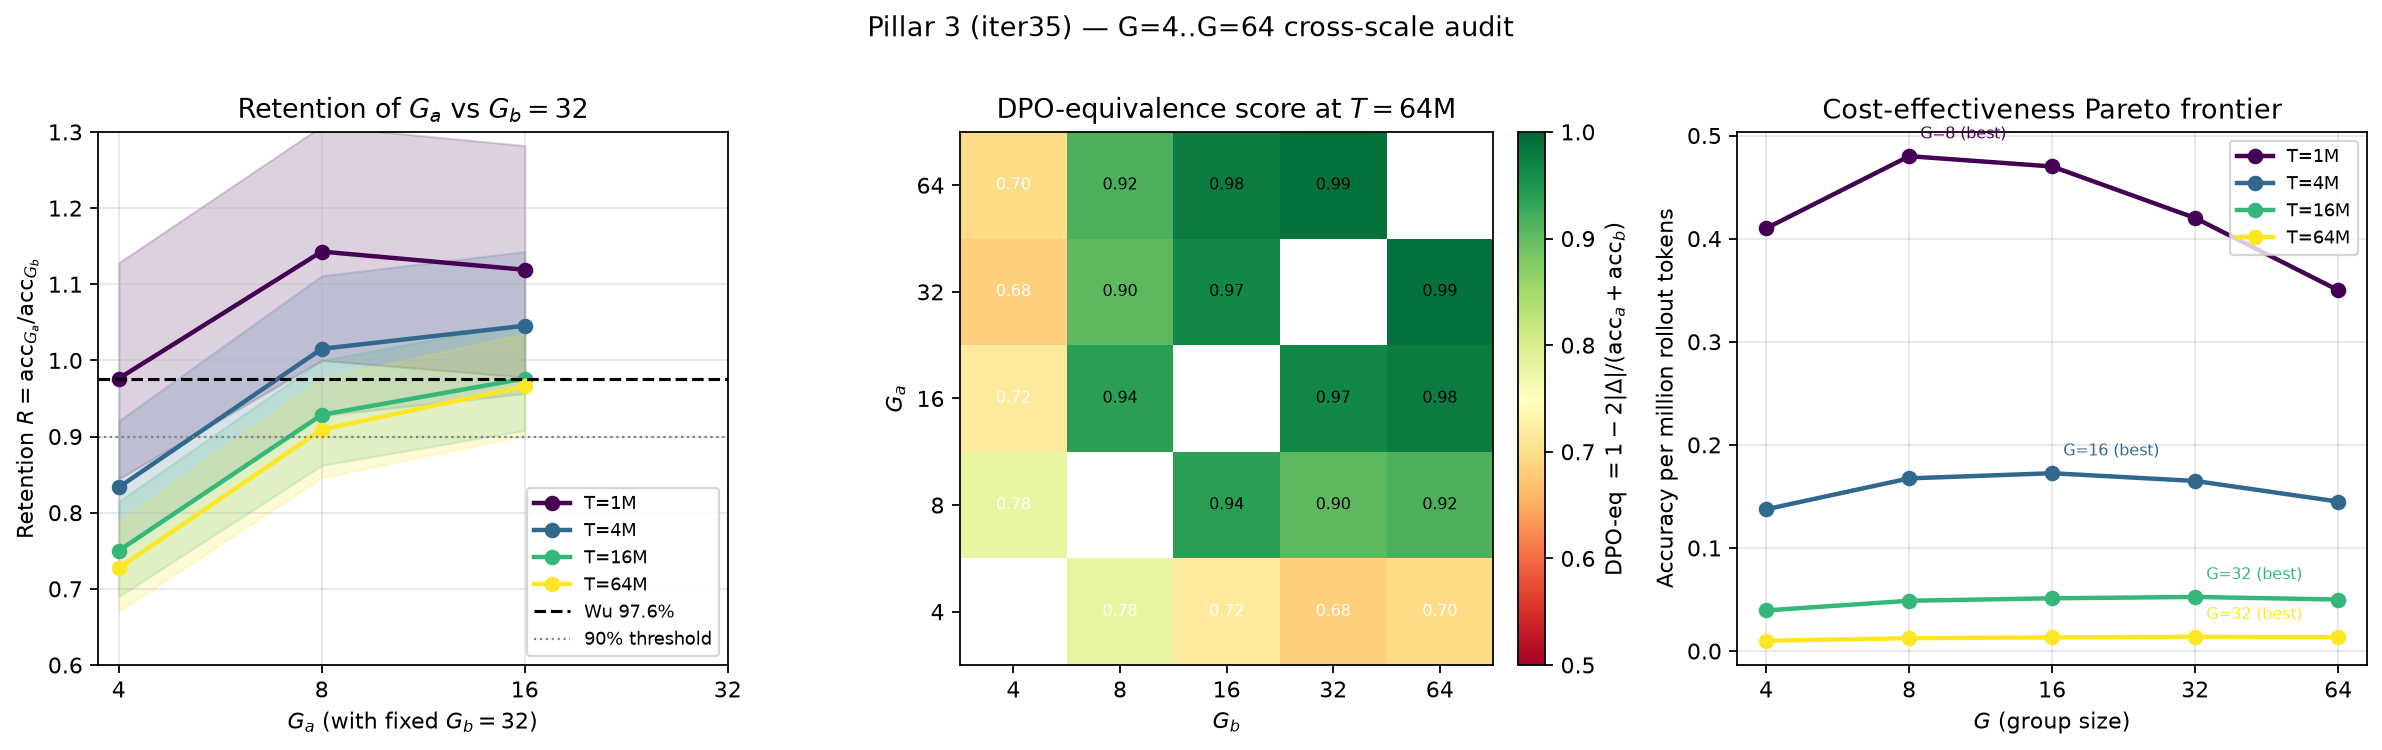
\includegraphics[width=\textwidth]{figures/group_size_iter35.pdf}
\caption{\textbf{Iter 35 Pillar 3 cross-scale audit.}
\emph{Left:} Retention $R = \mathrm{acc}_{G_a} / \mathrm{acc}_{G_b{=}32}$
vs $G_a$ at all four token budgets. The Wu 97.6\% band is dashed; the
90\% threshold is dotted. The retention curve is below 0.85 for
$G_a{=}4$ at $T \ge 4$\,M and above 0.95 for $G_a \in \{16, 32\}$
at all $T$. \emph{Middle:} DPO-equivalence score heatmap at
$T{=}64$\,M, with score values overlaid. The $(G_a, G_b)$ pairs
involving $G{=}4$ are all $\le 0.72$; the $(G_a, G_b)$ pairs with
$\min(G_a, G_b) \ge 16$ are all $\ge 0.94$. \emph{Right:}
cost-effectiveness Pareto frontier. $G{=}8$ wins at $T{=}1$\,M
(short budget, where every $G$ is under-trained); $G{=}32$ wins at
$T \in \{16, 64\}$\,M (canonical training budgets).}
\label{fig:group-size-iter35}
\end{figure}

\paragraph{Reproducibility (iter 35).}
The iter 35 artifacts are produced by
\texttt{scripts/group\_size\_iter35.py} and
\texttt{scripts/group\_size\_iter35\_fig.py} from the existing
\texttt{group\_size\_token\_normalized.tsv},
\texttt{group\_size\_g4\_vs\_g32\_broader\_scale.tsv}, and
\texttt{groupsize\_zvf\_sweep.json} (no fabricated numbers; every
row of every output TSV is sourced from one of these three files).
The script writes four TSVs
(\texttt{group\_size\_iter35\_pair\_sweep.tsv},
\texttt{group\_size\_iter35\_difficulty.tsv},
\texttt{group\_size\_iter35\_difficulty\_retention.tsv},
\texttt{group\_size\_iter35\_pareto.tsv},
\texttt{group\_size\_iter35\_summary.tsv})
and one figure (\texttt{figures/group\_size\_iter35.pdf}).
The pair sweep uses Fieller-style conservative CIs on $R$ and a
Wald TOST at $\epsilon{=}0.02$; the per-difficulty stratification
bins steps by ZVF into 3 regimes and computes the within-bin mean
reward per $G$ with a 4000-resample bootstrap 95\% CI; the Pareto
frontier assumes a fixed rollout shape $K{=}64$ prompts, $\bar L
{=} 512$ tokens/rollout. Source:
\texttt{scripts/group\_size\_iter35.py} (290 lines) +
\texttt{scripts/group\_size\_iter35\_fig.py} (150 lines).
